\graphicspath{{../../S22_Calculs_avec_des_fractions/Images/}}

\themeN
\chapter{Calculs avec des fractions}
\label{S22}

\programme%
   {\item Somme, différence de deux nombres rationnels.}
   {\item Calculer avec des fractions.
    \item Effectuer des calculs et des comparaisons pour traiter des problèmes.}

\vfill

\begin{debat}{Débat : l'\oe il d'Oudjat, ou \oe il d'Horus}
   Dans la mythologie égyptienne, on trouve une histoire liée aux fractions : {\it Seth}, dieu de la violence et incarnation du mal, aurait arraché l’{\bf œil} à {\bf Horus}. {\it Seth} l'aurait partagé en six morceaux et les aurait répandu à travers l’Égypte. {\it Thot}, dieu magicien, aurait reconstitué l’\oe il, symbole du bien contre le mal. On dit que chacune de ses parties symbolise une fraction de numérateur 1 et de dénominateurs 2, 4, 8, 16, 32 et 64 et qu'il accordera le 64\up{e} manquant à tout scribe recherchant et acceptant sa protection.
   \tcblower
      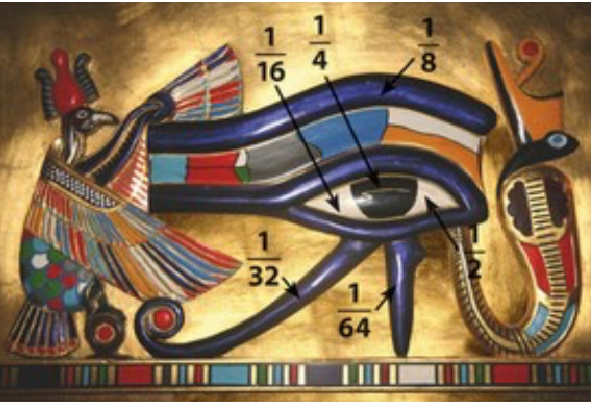
\includegraphics[width=6cm]{Horus}
\end{debat}

\hfill {\gray Vidéo : \href{https://www.youtube.com/watch?v=TTLRP1Yd4Wk&embeds_referring_euri=https%3A%2F%2Fwww.arieka.fr%2F&source_ve_path=Mjg2NjY&feature=emb_logo}{\bf Addition et soustraction de fractions}, chaîne YouTube {\it Rapémathiques}, d'A'Rieka.}


%%% Approche %%%
\begin{Maquette}[Cours]{Theme={Activité d'approche},Couleur={SteelBlue}}

   \AAtitre{Décomposer une fraction}

   {\it Objectifs : représenter des fractions ; écrire une fraction sous la forme de la somme ou de la différence d'un entier et d'une fraction inférieure à 1.}

      \begin{AActivite}

         \AApartie{Des toasts en entrée}
            Pour faire des toasts à ses amis, Clara coupe des tranches de pain de mie en quatre, avant de les garnir. \par
            Narmin mange onze de ces petits toasts. Elle a mangé 11 fois $\dfrac14$ de grande tranche, donc $\dfrac{11}4$ de grande tranche.
            \begin{center}
               \Fraction[Rectangle,Longueur=2cm,Largeur=1.5cm,Multiple=2,Couleur=1.2SteelBlue,Reponse]{11/4}
               \qquad
               \Fraction[Rectangle,Longueur=2cm,Largeur=1.5cm,Multiple=2]{8/4}
            \end{center}
            Ce qui fait 2 tranches et $\dfrac34$ de tranche, ou 3 tranches moins $\dfrac14$ de tranche. On écrit : $\dfrac{11}{4} =2+\dfrac34 =3-\dfrac14$. \par \smallskip
            Aboubaker, lui, a mangé 17 petits toasts. Colorier ce que cela représente ci-dessous.
            \begin{center}
               \Fraction[Rectangle,Longueur=2cm,Largeur=1.5cm,Multiple=2]{17/4}
            \end{center}
            \smallskip
            Compléter l'égalité  : \quad $\dfrac{17}{4} = \pointilles[1cm] + \dfrac{\pointilles[1cm]}{\pointilles[1cm]} =\pointilles[1cm] - \dfrac{\pointilles[1cm]}{\pointilles[1cm]}$

      \AApartie{Des \og flam \fg{} en plat principal}
         Pour poursuivre, Clara propose à ses amis de manger des flammekueches (flam). \par
         \begin{center}
            \Fraction[Rayon=8mm,Couleur=1.2SteelBlue,Reponse]{8/5} \qquad \Fraction[Rayon=8mm]{8/5}
         \end{center}
         Proportion de flam mangée : $\dfrac{\pointilles[1cm]}{\pointilles[1cm]} ={\pointilles[1cm]} + \dfrac{\pointilles[1cm]}{\pointilles[1cm]} ={\pointilles[1cm]} - \dfrac{\pointilles[1cm]}{\pointilles[1cm]}$ \par \bigskip
         Colorier $\dfrac{13}{8}$ de flam : \qquad \raisebox{-4mm}{\Fraction[Rayon=8mm]{32/8}} \par \bigskip
         Compléter l'égalité  : \quad $\dfrac{13}{8} ={\pointilles[1cm]} + \dfrac{\pointilles[1cm]}{\pointilles[1cm]} ={\pointilles[1cm]} - \dfrac{\pointilles[1cm]}{\pointilles[1cm]}$ \par \bigskip

      \AApartie{Des éclairs en dessert}
         Narmin a mangé $\dfrac{73}9$ de mini-éclairs au chocolat, trouver une manière de décomposer cette fraction en la somme et la différence d'un nombre entier et d'une fraction inférieure à 1. \par
         \vspace*{1.8cm}

      \end{AActivite}

   \vfill\hfill{\it\footnotesize Source : Inspiré de \href{http://ww2.ac-poitiers.fr/dsden86-pedagogie/sites/dsden86-pedagogie/IMG/pdf/groupe4_c13.pdf}{\og Écrire une fraction sous la forme d'un entier et d'une fraction inférieure à 1 \fg}, académie de Poitiers.}

\end{Maquette}


%%%Trace écrite %%%
\begin{Maquette}[Cours]{Theme={Trace écrite},Couleur={0.4[SteelBlue,Black]}}

   %%%1
   \section{Décomposer une fraction}
  
      \begin{methode*}{Décomposer une fraction}
         Pour décomposer une fraction en somme ou différence d'un entier et d'une fraction inférieure à 1, on peut effectuer la division euclidienne du numérateur par le dénominateur. 
         \begin{itemize}
            \item Pour une somme, le quotient nous donne le nombre entier et la fraction inférieure à 1 s'obtient en prenant comme numérateur le reste et comme dénominateur le diviseur.
            \item Pour une différence, il suffit de prendre l'entier suivant le quotient et de choisir la fraction complémentaire à 1.
         \end{itemize}
         \begin{exbmethode}
            Décomposer $\dfrac{23}{6}$.
            \tcblower
               $\opidiv{23}{6}$
               \qquad $\raisebox{-4mm}{\Fraction[Rayon=6.5mm,Couleur=Crimson,Reponse]{23/6}}$
               \qquad $\dfrac{23}{6} =3+\dfrac56 =4-\dfrac16$
            \end{exbmethode}
      \end{methode*}


   %%%2
   \section{Additionner et soustraire des fractions} %%%

      \begin{methode*}{même dénominateur}
         Pour additionner ou soustraire deux fractions ayant le même dénominateur, il suffit d'additionner ou de soustraire les numérateurs tout en gardant le même dénominateur :
         $${a\over c}+{b\over c}={a+b\over c} \qquad \text{et} \qquad {a\over c}-{b\over c}={a-b\over c}$$ \vspace*{-12mm}
         \begin{exbmethode}
            \begin{multicols}{2}
               Additionner $\dfrac36$ et $\dfrac26$.  \par
               Soustraire $\dfrac26$ de $\dfrac36$.
            \end{multicols}
            \tcblower
               \begin{multicols}{2}
                  $\dfrac36+\dfrac26 =\dfrac{3+2}{6} =\dfrac56$
                  \quad $\raisebox{-4mm}{\Fraction[Rayon=5mm,Couleur=Crimson,Reponse]{3/6}} + \raisebox{-4mm}{\Fraction[Rayon=5mm,Couleur=Crimson,Reponse]{2/6}} = \raisebox{-4mm}{\Fraction[Rayon=5mm,Couleur=Crimson,Reponse]{5/6}}$ \par
                  $\dfrac36-\dfrac26 =\dfrac{3-2}{6} =\dfrac16$
                  \quad $\raisebox{-4mm}{\Fraction[Rayon=5mm,Couleur=Crimson,Reponse]{3/6}} - \raisebox{-4mm}{\Fraction[Rayon=5mm,Couleur=Crimson,Reponse]{2/6}} = \raisebox{-4mm}{\Fraction[Rayon=5mm,Couleur=Crimson,Reponse]{1/6}}$
               \end{multicols}
        \end{exbmethode}
      \end{methode*}

      \smallskip

      \begin{methode*}{dénominateurs multiples}
         Pour additionner ou soustraire deux fractions ayant des dénominateurs multiples, on transforme l'écriture d'une fraction pour qu'elle ait le même dénominateur que l'autre.
         \begin{exbmethode}
            \begin{multicols}{2}
               Additionner $\dfrac23$ et $\dfrac56$. \par
               Soustraire $\dfrac23$ de $\dfrac{11}{12}$.
            \end{multicols}
            \tcblower
               $\dfrac23+\dfrac56 =\dfrac{2\times2}{2\times3}+\dfrac56 =\dfrac46+\dfrac56 =\dfrac96$    
               \hskip1.2cm $\raisebox{-4mm}{\Fraction[Rayon=5.5mm,Couleur=Crimson,Reponse]{2/3}} + \raisebox{-4mm}{\Fraction[Rayon=5.5mm,Couleur=Crimson,Reponse]{5/6}} = \raisebox{-4mm}{\Fraction[Rayon=5.5mm,Couleur=Crimson,Reponse]{4/6}} + \raisebox{-4mm}{\Fraction[Rayon=5.5mm,Couleur=Crimson,Reponse]{5/6}} = \raisebox{-4mm}{\Fraction[Rayon=5.5mm,Couleur=Crimson,Reponse]{6/6} \Fraction[Rayon=5.5mm,Couleur=Crimson,Reponse]{3/6}}$ \par \bigskip
               $\dfrac{11}{12}-\dfrac23 =\dfrac{11}{12}-\dfrac{4\times2}{4\times3} =\dfrac{11}{12}-\dfrac{8}{12} =\dfrac3{12}$
               \quad $\raisebox{-4mm}{\Fraction[Rayon=5.5mm,Couleur=Crimson,Reponse]{11/12}} - \raisebox{-4mm}{\Fraction[Rayon=5.5mm,Couleur=Crimson,Reponse]{2/3}} = \raisebox{-4mm}{\Fraction[Rayon=5.5mm,Couleur=Crimson,Reponse]{11/12}} - \raisebox{-4mm}{\Fraction[Rayon=5.5mm,Couleur=Crimson,Reponse]{8/12}} = \raisebox{-4mm}{\Fraction[Rayon=5.5mm,Couleur=Crimson,Reponse]{3/12}}$
            \end{exbmethode}
      \end{methode*}

      Remarque : cela revient à dire que pour additionner ou soustraire des parts, il faut auparavant qu'elles soient égales, et donc partager les parts les plus grandes de manière à ce qu'elles aient la même taille que les parts les plus petites.

\end{Maquette}


%%% Exercices %%%
\begin{Maquette}[Fiche,CorrigeFin,Colonnes=2]{}

   \begin{multicols}{2}

      \begin{exercice} %1
         Écrire chaque fraction sous la forme de la somme d'un nombre entier et d'une fraction inférieure à 1 en faisant le calcul mentalement. En déduire une écriture comme la soustraction d'un entier et d'une fraction. \medskip
         \begin{colenumerate}[3]
            \item $\dfrac72$ \medskip
            \item $\dfrac98$
            \item $\dfrac13$
            \item $\dfrac53$
            \item $\dfrac{11}{4}$
            \item $\dfrac{13}{4}$
         \end{colenumerate}
      \end{exercice}
      
      \begin{Solution}
         \begin{colenumerate}
            \item $\dfrac72 =\cor{3+\dfrac12 =4-\dfrac12}$
            \item $\dfrac98 =\cor{1+\dfrac18 =2-\dfrac78}$
            \item $\dfrac13 =\cor{0+\dfrac13 =1-\dfrac23}$
            \item $\dfrac53 =\cor{1+\dfrac23 =2-\dfrac13}$
            \item $\dfrac{11}{4} =\cor{2+\dfrac34 =3-\dfrac14}$
            \item $\dfrac{13}{4} =\cor{3+\dfrac14 =4-\dfrac34}$
         \end{colenumerate}
      \end{Solution}
      
      
      \begin{exercice} %2
         Écrire chaque fraction sous la forme de la somme d'un nombre entier et d'une fraction inférieure à 1 en posant la division euclidienne. En déduire une écriture comme la soustraction d'un entier et d'une fraction. \medskip
         \begin{colenumerate}[3]
            \item $\dfrac{27}2$ \medskip
            \item $\dfrac{92}8$
            \item $\dfrac{13}{3}$
            \item $\dfrac{53}{3}$
            \item $\dfrac{121}{5}$
            \item $\dfrac{127}{4}$
         \end{colenumerate}
      \end{exercice}
      
      \begin{Solution}
         \begin{enumerate}
            \item \opidiv[voperation=top]{27}{2} donc, $\dfrac{27}2 =\cor{13+\dfrac12 =14-\dfrac12}$
            \item \opidiv[voperation=top]{92}{8} donc, $\dfrac{92}8 =\cor{11+\dfrac48 =12-\dfrac48}$
            \item \opidiv[voperation=top]{13}{3} donc, $\dfrac{13}{3} =\cor{4+\dfrac13 =5-\dfrac23}$
            \item \opidiv[voperation=top]{53}{3} donc, $\dfrac{53}{3} =\cor{17+\dfrac23 =18-\dfrac13}$
            \item \opidiv[voperation=top]{121}{5} donc, $\dfrac{121}{5} =\cor{24+\dfrac15 =25-\dfrac45}$
            \item \opidiv[voperation=top]{127}{4} donc, $\dfrac{127}{4} =\cor{31+\dfrac34 =32-\dfrac14}$
         \end{enumerate}
      \end{Solution}
      
      
      \begin{exercice} %3
         Dans cet exercice, l'unité est le carré suivant (le tangram), constitué de sept pièces. \par
         {\psset{unit=1.7}
         \begin{pspicture}(-0.5,-0.2)(4,4.2)
            \psgrid[subgriddiv=1,gridcolor=gray!80,gridlabels=0](4,4)
            \psset{linewidth=0.5mm}
            \psframe(0,0)(4,4)
            \psline(0,0)(4,4)
            \psline(3,1)(0,4)
            \psline(2,0)(4,2)
            \psline(2,0)(1,1)
            \psline(3,1)(3,3)
            \rput(0.8,2){\large 5}
            \rput(2,3.2){\large 6}
            \rput(1,0.4){\large 2}
            \rput(2,1){\large 1}
            \rput(2.6,2){\large 3}
            \rput(3.5,2.5){\large 4}
            \rput(3.5,0.6){\large 7}
         \end{pspicture}}
         \begin{enumerate}
            \item Quelle fraction du tangram représente chacune des pièces de 1 à 7 ?
            \item Avec quelles pièces du tangram (deux minimum) peut-on faire la fraction $\dfrac18$ ? \smallskip
            \item Avec quelles pièces (deux minimum) peut-on faire la fraction $\dfrac{3}{16}$ ? Donner trois possibilités. \smallskip
            \item Avec quelles pièces (deux minimum) peut-on faire la fraction $\dfrac14$ ? Donner quatre possibilités.
         \end{enumerate}
      \end{exercice}
      
      \begin{Solution}
         \begin{enumerate}
            \item Les pièces 2 et 3 représentent \cor{$\dfrac{1}{16}$} du tangram. \par
               Les pièces 1, 4 et 7 représentent \cor{$\dfrac18$} du tangram. \par
               Les pièces 5 et 6 représentent \cor{$\dfrac14$} du tangram.
            \item On peut faire $\dfrac18$ avec les pièces \cor{2 et 3}.
            \item On peut faire $\dfrac{3}{16}$ avec les pièces  \par
               \cor{1 et 2} ou \cor{1 et 3} ou encore \cor{3 et 4}.
            \item On peut faire $\dfrac14$ avec les pièces  \par
               \cor{4 et 7} ou \cor{1, 2 et 3} ou \cor{2, 3 et 4} encore \cor{1 et 4}.
         \end{enumerate}
      \end{Solution}

      
      \begin{exercice} %4
         Effectuer les calculs suivants puis simplifier. \medskip
         \begin{colenumerate}
            \item $\dfrac23+\dfrac73$ \medskip
            \item $\dfrac67-\dfrac37$ \medskip
            \item $\dfrac3{13}-\dfrac8{13}$ \medskip
            \item $\dfrac12+\dfrac32+\dfrac52$
            \item $\dfrac{12}7+\dfrac27-\dfrac97$
            \item $\dfrac8{10}-\dfrac{302}{10}+\dfrac{78}{10}$
         \end{colenumerate}
      \end{exercice}
      
      \begin{Solution}
         \begin{enumerate}
            \item $\dfrac23+\dfrac73 =\dfrac{2+7}{3} =\dfrac93 =\cor{3}$
            \item $\dfrac67-\dfrac37 =\dfrac{6-3}{7} =\cor{\dfrac37}$
            \item $\dfrac3{13}-\dfrac8{13} =\dfrac{3-8}{13} =\dfrac{-5}{13} =\cor{-\dfrac{5}{13}}$
            \item $\dfrac12+\dfrac32+\dfrac52 =\dfrac{1+3+5}{2} =\cor{\dfrac92}$
            \item $\dfrac{12}7+\dfrac27-\dfrac97 =\dfrac{12+2-9}{7} =\cor{\dfrac{5}{7}}$
            \item $\dfrac8{10}-\dfrac{302}{10}+\dfrac{78}{10} =\dfrac{8-302+78}{10} =\dfrac{-216}{10} =\cor{-\dfrac{108}{5}}$
         \end{enumerate}
      \end{Solution}
      
      
      \begin{exercice} %5
         Répondre aux petits défis suivants :
         \begin{enumerate}
            \item Combien faut-il ajouter à $\dfrac23$ pour obtenir 1 ? \smallskip
            \item Combien faut-il soustraire à $\dfrac{15}4$ pour obtenir 3 ? \smallskip
            \item Combien faut-il ajouter à $\dfrac{13}{10}$ pour obtenir 2 ? \smallskip
            \item Combien faut-il soustraire à $\dfrac{52}{17}$ pour obtenir 3 ?
         \end{enumerate}
      \end{exercice}
      
      \begin{Solution}
         \begin{enumerate}
            \item Il faut ajouter $\cor{\dfrac13}$ à $\dfrac23$ pour obtenir 1.
            \item $\dfrac{15}{4} =3+\dfrac34$ donc, \par
               il faut soustraire $\cor{\dfrac34}$ à $\dfrac{15}{4}$ pour obtenir 3.
            \item $\dfrac{13}{10} =1+\dfrac{3}{10}$ donc, \par
               il faut ajouter $\cor{\dfrac{7}{10}}$ à $\dfrac{13}{10}$ pour obtenir 2.
            \item $\dfrac{52}{17} =3+\dfrac{1}{17}$ donc, \par
               il faut soustraire $\cor{\dfrac{1}{17}}$ à $\dfrac{52}{17}$ pour obtenir 3.
         \end{enumerate}
      \end{Solution}
      
      
      \begin{exercice}[Dur] %6
         Effectuer les calculs suivants, puis simplifier. \smallskip
         \begin{colenumerate}
            \item $\dfrac23+\dfrac76$ \smallskip
            \item $\dfrac67-\dfrac3{14}$ \smallskip
            \item $\dfrac{38}{13}-\dfrac3{39}$ \smallskip
            \item $\dfrac{18}{46}+\dfrac{28}{23}$ \smallskip
            \item $\dfrac83-\dfrac26-\dfrac4{12}$
            \item $\dfrac12+\dfrac34+\dfrac58$
            \item $\dfrac34-4-\dfrac5{16}$
            \item $\dfrac{12}{49}+2-\dfrac97$
         \end{colenumerate}
      \end{exercice}
      
      \begin{Solution}
         \begin{enumerate}
            \item $\dfrac23+\dfrac76 =\dfrac46+\dfrac76 =\cor{\dfrac{11}6}$
            \item $\dfrac67-\dfrac3{14} =\dfrac{12}{14}-\dfrac3{14} =\cor{\dfrac9{14}}$
            \item $\dfrac{38}{13}-\dfrac3{39} =\dfrac{114}{39}-\dfrac3{39} =\dfrac{111}{39} =\cor{\dfrac{37}{13}}$
            \item $\dfrac{18}{46}+\dfrac{28}{23} =\dfrac{9}{23}+\dfrac{28}{23} =\cor{\dfrac{37}{23}}$
            \item $\dfrac83-\dfrac26-\dfrac4{12} =\dfrac{32}{12}-\dfrac{4}{12}-\dfrac{4}{12} =\dfrac{24}{12} =\cor{2}$
            \item $\dfrac12+\dfrac34+\dfrac58 =\dfrac48+\dfrac68+\dfrac58 =\cor{\dfrac{15}{8}}$
            \item $\dfrac34-4-\dfrac5{16} =\dfrac{12}{16}-\dfrac{64}{16}-\dfrac{5}{16} =\cor{-\dfrac{57}{16}}$
            \item $\dfrac{12}{49}+2-\dfrac97 =\dfrac{12}{49}+\dfrac{98}{49}-\dfrac{63}{49} =\cor{\dfrac{47}{49}}$
         \end{enumerate}
      \end{Solution}

      
      \begin{exercice}[Dur] %7
         Un adulte passe en moyenne 25\,\% de son temps à travailler, $\dfrac13$ à dormir, $\dfrac{1}{12}$ à gérer le quotidien et $\dfrac{3}{36}$ à manger.
         \begin{enumerate}
            \item Sur une journée de 24 heures, combien de temps un adulte passe-t-il sur chacune de ces activités ?
            \item Quelle pourcentage de son temps lui reste-t-il pour ses loisirs ?
         \end{enumerate}
      \end{exercice}
      
      \begin{Solution}
         \begin{enumerate}
            \item Sur une journée, un adulte passe : \smallskip
            \begin{itemize}
               \item 25\,\% correspond à une faction de $\dfrac14$. \par
                  \quad $\dfrac14\times\Temps{;;;24} =$ \cor{\Temps{;;;6} pour travailler} ; \par
               \item $\dfrac13\times\Temps{;;;24} =$ \cor{\Temps{;;;8} pour dormir} ; \par
               \item $\dfrac1{12}\times\Temps{;;;24} =$ \cor{\Temps{;;;2} pour gérer le quotidien} ; \par
               \item $\dfrac{3}{36}\times\Temps{;;;24} =$ \cor{\Temps{;;;2} pour manger.}
            \end{itemize}
            \item On calcule le nombre d'heures restantes : \par
               $\Temps{;;;24}-\Temps{;;;6}-\Temps{;;;8}-\Temps{;;;2}-\Temps{;;;2} =\Temps{;;;6}$. \par
               Or, $\dfrac{\Temps{;;;6}}{\Temps{;;;24}} =\dfrac{1\times\Temps{;;;6}}{4\times\Temps{;;;6}} =\dfrac14 =25\,\%$. \par
               \cor{Il lui reste donc 25\,\% de son temps pour les loisirs}.
         \end{enumerate} 
      \end{Solution}
      

      \begin{exercice} %8
         Pour chaque figure, exprimer la partie coloriée à l'aide d'une fraction de la surface du grand carré.
         \begin{center}
            \begin{pspicture}(0,-0.3)(2,2)
               \psframe(0,0)(2,2)
               \psline(1,0)(1,1)(1.5,0.5)(2,1)
               \psset{fillstyle=solid,fillcolor=Crimson}
               \psframe(1,1)(2,2)
               \pspolygon(0,0)(1,1)(0,1)
               \pspolygon(1,0)(2,0)(1.5,0.5)
               \rput(1,-0.3){figure 1}
            \end{pspicture}
            \quad
            \begin{pspicture}(0,-0.3)(2,2)
               \psframe(0,0)(2,2)
               \psline(0.67,0)(0.67,0.67)
               \psline(1,0.67)(1.33,0.67)
               \psset{fillstyle=solid,fillcolor=DodgerBlue}
               \psframe(0,1.33)(2,2)
               \psframe(0,0.67)(1,1.33)
               \psframe(1.33,0)(2,0.67)
               \rput(1,-0.3){figure 2}
            \end{pspicture}
            \quad
            \begin{pspicture}(0,-0.3)(2,2)
               \psframe(0,0)(2,2)
               \psline(1,1.5)(1,1)(2,2)
               \psset{fillstyle=solid,fillcolor=DarkOrange}
               \pspolygon(0,0)(1,1)(0,2)
               \pspolygon(1,0)(1,1)(2,0)
               \pspolygon(1,1)(2,1)(1.5,1.5)
               \pspolygon(1,1.5)(1,2)(0.5,1.5)
               \rput(1,-0.3){figure 3}
            \end{pspicture}
         \end{center}
      \end{exercice}
      
      \begin{Solution}
         On peut dessiner un quadrillage par-dessus la figure afin de \og compter \fg{} les parties colorées ou additionner les fractions. \par
         Figure 1 : $\dfrac14+\dfrac18+\dfrac{1}{16} =\dfrac{4}{16}+\dfrac{2}{16}+\dfrac{1}{16} =\cor{\dfrac{7}{16}}$ \par
         Figure 2 : $\dfrac13+\dfrac16+\dfrac19 =\dfrac{6}{18}+\dfrac{3}{18}+\dfrac{2}{18} =\cor{\dfrac{11}{18}}$ \par
         figure 3 : $\dfrac14+\dfrac18+\dfrac{1}{16}+\dfrac{1}{32} =\dfrac{8}{32}+\dfrac{4}{32}+\dfrac{2}{32}+\dfrac{1}{32} =\cor{\dfrac{15}{32}}$
      \end{Solution}

   \end{multicols}

\end{Maquette}


%%% Récré %%%
\begin{Maquette}[Cours]{Theme={Activité récréative},Couleur={IndianRed}}
    
   \ARtitre{Sudofractions}

      \begin{minipage}{7cm}
         \begin{itemize}
            \item Calculer la somme ou la différence proposée dans chaque case de la grille ci-dessous.
            \item Simplifier la fraction si possible.
            \item Choisir le numérateur de la fraction obtenue et le reporter dans la case correspondante de la grille vierge de sudoku ci-contre.
            \item Compléter la grille selon les règles du Sudoku.
         \end{itemize}
         {\it Par exemple, $\dfrac96-\dfrac56 =\dfrac46 =\dfrac{\textbf{2}}{3}$ donc, la troisième \par \smallskip
         case de la ligne du haut comporte un 2}.
      \end{minipage}
      \qquad
      \begin{minipage}{10cm}
      {\hautab{2}
         \begin{tabular}{|*{3}{C{0.6}|}|*{3}{C{0.6}|}|*{3}{C{0.6}|}}
            \hline
            & & {\bf 2} & & & & & & \\
            \hline
            & & & & & & & & \\
            \hline
            & & & & & & & & \\
            \hline
            \hline
            & & & & & & & & \\
            \hline
            & & & & & & & & \\
            \hline
            & & & & & & & & \\
            \hline
            \hline
            & & & & & & & & \\
            \hline
            & & & & & & & & \\
            \hline
            & & & & & & & & \\
            \hline
         \end{tabular}}
      \end{minipage}
      \vfill
      \begin{center}
      {\hautab{3.6}\footnotesize
         \begin{tabular}{|*{3}{C{1}|}|*{3}{C{1}|}|*{3}{C{1}|}}
            \hline
               \!$\dfrac1{13}+\dfrac5{13}$\! & $\dfrac17+\dfrac47$ & $\dfrac96-\dfrac56$ & & $\dfrac43+\dfrac43$ & $\dfrac84-\dfrac14$ & $\dfrac32+\dfrac62$ & & \!$\dfrac{15}{14}-\dfrac{7}{14}\!$ \\
            \hline
               $\dfrac23+\dfrac53$ & $\dfrac12+\dfrac24$ & & $\dfrac59-\dfrac19$ & & & $\dfrac57-\dfrac27$ & & \\
            \hline
               & & $\dfrac53+\dfrac33$ & $\dfrac56-\dfrac13$ & & & & & $\dfrac52+1$\\
               \hline
               \hline
               $\dfrac{12}7-\dfrac47$ & $1-\dfrac13$ & & & $\dfrac15+\dfrac{1}{10}$ & & & & $\dfrac37+\dfrac37$ \\
            \hline
               $1+\dfrac23$ & & & $\dfrac59-\dfrac13$ & & & & $\dfrac12+\dfrac14$ & \\
            \hline
               & & & $\dfrac{14}{9}-\dfrac23$ & & & $\dfrac43+\dfrac13$ & $\dfrac52-\dfrac12$ & \\
            \hline
            \hline
               & $1-\dfrac19$ & $\dfrac38+\dfrac12$ & $\dfrac32-\dfrac14$ & $\dfrac{11}3-\dfrac93$ & & $\dfrac62+\dfrac{12}4$ & $\dfrac36+\dfrac56$ & \\
            \hline
               \!$\dfrac{12}{11}-\dfrac{10}{11}$\! & $\dfrac72-\dfrac{25}{8}$ &  & $1-\dfrac17$ & & $\dfrac97-\dfrac17$ & & $\dfrac27+1$ & \\
            \hline
               $2+\dfrac52$ & & & & $\dfrac17+\dfrac37$ & & & & \\
            \hline
         \end{tabular}}
      \end{center}

\end{Maquette}